\documentclass[a4paper]{article}

\usepackage{amsmath}
\usepackage{amssymb}
\usepackage[margin=1.5cm,
            includefoot,
            footskip=30pt]{geometry}
\usepackage{layout}
\usepackage{graphicx}
\usepackage{subcaption}

\usepackage{biblatex}
\usepackage{pdfpages}
\usepackage{booktabs}

\bibliography{main.bib}

\title{Suspicion: Recognising and evaluating the effectiveness
       of extortion in the Iterated Prisoner's Dilemma}
\author{Vincent A. Knight \and Nikoleta E. Glynatsi}
\date{\today}



\begin{document}

\maketitle

\begin{abstract}
    The Iterated Prisoner's Dilemma is a model for rational and evolutionary
    interactive behaviour. It has applications both in the study of human social
    behaviour as well as in biology.
    It is used to understand when and how a rational individual might
    accept an immediate cost to their own utility for the direct benefit of
    another.

    Much attention has been given to a class of strategies called
    Zero Determinant strategies. It has been theoretically shown that these
    strategies can ``extort'' any player.

    In this work, an approach to identify if observed strategies are playing in
    an extortionate way is described. Furthermore, experimental analysis of
    a large tournament with 204
    strategies is considered. In this setting
    the most highly performing strategies do not play in an extortionate way
    against each other but do against lower performing strategies.
    This suggests that whilst the theory of Zero Determinant strategies
    indicates that memory is not of fundamental importance to the evolution of
    cooperative behaviour, this is incomplete.
\end{abstract}

\section{Introduction}\label{sec:introduction}

Agent based game theoretic models have become a stalwart of the underpinning
mathematics of interactive behaviours. One of the major pieces of work
in this area is the pair of original computer tournaments run by Robert
Axelrod~\cite{Axelrod1980, Axelrod1980a}. These tournaments pitted submitted
computer strategies against each other in plays of the Iterated Prisoner's
Dilemma. A common game where agents can choose to pay a slight cost to their
immediate utility in the hope of building a reputation. This has been used in
economic and evolutionary game theory to understand the evolution of cooperative
behaviour.

Recently, a class of strategies was described in~\cite{Press2012} that can
provably extort any given opponent. In~\cite{Hilbe2013, Moran1707} some
questions have already been asked about the true effectiveness of these
strategies in an evolutionary setting. Here another question is asked: is it
possible to recognise this extortionate behaviour? A mathematical procedure for
suspicion is presented: in the same way that the continued actions of an
extortionate individual might raise suspicion.

This work makes use of the Axelrod Python library~\cite{Knight2016, Knight2018}
with a large number of Prisoner Dilemma strategies available to give an
extensive numerical example of the ideas presented.  The approach is presented
in Section~\ref{sec:delta-zd-strategies}.  All of the code and data discussed
in Section~\ref{sec:numerical-experiments} is open sourced, archived and
written according to best scientific principles~\cite{Wilson2014}. The data
archive can be found at~\cite{vincent_knight_2018_1297075}.

\section{Recognising Extortion}\label{sec:delta-zd-strategies}

In~\cite{Press2012}, given a match between 2 memory one strategies, the concept
of Zero Determinant (ZD) strategies is introduced. The main result of that paper
shows that given two memory one players \(p, q\in\mathbb{R}^4\) a linear
relationship between the players' scores could be forced by one of the players.

Using the notation of~\cite{Press2012}, assuming the utilities for player \(p\)
are given by \(S_x=(R, S, T, P)\) and for player \(q\) by \(S_y=(R, T, S, P)\)
and that the stationary scores of each player is given by \(S_X\) and \(S_Y\)
respectively. The main result of~\cite{Press2012} is that if

\begin{equation}\label{eqn:linear_relationship_for_p}
    \tilde p=\alpha S_x + \beta S_y + \gamma
\end{equation}

or

\begin{equation}\label{eqn:linear_relationship_for_q}
    \tilde q=\alpha S_x + \beta S_y + \gamma
\end{equation}

where \(\tilde p = (1 - p_1, 1 - p_2, p_3, p_4)\) and
\(\tilde q = (1 - q_1, 1 - q_2, q_3, q_4)\) then:

\begin{equation}
    \alpha S_X + \beta S_Y + \gamma = 0
\end{equation}

In~\cite{Press2012} a particular type of ZD strategy is defined: extortionate
strategies. If:

\begin{equation}\label{eqn:constraint_for_extortion}
    \gamma = - P(\alpha + \beta)
\end{equation}

then the player can ensure they get a score \(\chi\) times
larger than the opponent. This extortion coefficient is given by:

\begin{equation}\label{eqn:definition_of_chi}
    \chi=\frac{-\beta}{\alpha}
\end{equation}

Thus, if (\ref{eqn:constraint_for_extortion}) holds and \(\chi >1\) a player is
said to extort their opponent.
Here, the reverse problem is considered: given a
\(p\in\mathbb{R}^4\) how does one identify \(\alpha, \beta\) if they
exist and is the strategy in fact acting in an extortionate way?

In this case constraints (\ref{eqn:linear_relationship_for_p}) and
(\ref{eqn:constraint_for_extortion}) correspond to:

\begin{align}
    \tilde p_1 & = \alpha R + \beta R - P (\alpha + \beta)
            \label{eqn:condition_for_tilde_p1}\\
    \tilde p_2 & = \alpha S + \beta T - P (\alpha + \beta)
            \label{eqn:condition_for_tilde_p2}\\
    \tilde p_3 & = \alpha T + \beta S - P (\alpha + \beta)
            \label{eqn:condition_for_tilde_p3}\\
    \tilde p_4 & = \alpha P + \beta P - P (\alpha + \beta)
            \label{eqn:condition_for_tilde_p4}
\end{align}

Equation (\ref{eqn:condition_for_tilde_p4}) ensures that \(p_4=\tilde p_4=0\).
Equations (\ref{eqn:condition_for_tilde_p1}-\ref{eqn:condition_for_tilde_p3})
can be used to eliminate \(\alpha, \beta\), giving:

\begin{equation}\label{eqn:planar_definition_of_extortion}
    \tilde p_1 = \frac{(R - P)(\tilde p_2 + \tilde p_3)}{S + T - 2P}
\end{equation}

with:

\begin{equation}\label{eqn:definition_of_chi}
    \chi = \frac{\tilde p_2 (P - T) + \tilde p_3 (S - P)}
                {\tilde p_2 (P - S) + \tilde p_3 (T - P)}
\end{equation}

Given a strategy \(p\in\mathbb{R}^{4}\) equations
(\ref{eqn:condition_for_tilde_p4}), (\ref{eqn:planar_definition_of_extortion}-\ref{eqn:definition_of_chi}) can be used to check if
a strategy is extortionate. The conditions correspond to:

\begin{align}
    p_1 & = \frac{(R-P)(p_2 + p_3) - R + T + S - P}{S + T - 2P}
     \label{eqn:condition_for_p1}\\
    p_4 & = 0 \label{eqn:condition_for_p4}\\
    1 & > p_2 + p_3\label{eqn:condition_for_chi}
\end{align}

The algebraic steps necessary to prove these results are available in the
supporting materials.

All extortionate strategies reside on a triangular (\ref{eqn:condition_for_chi})
plane (\ref{eqn:condition_for_p1}) in 3 dimensions (\ref{eqn:condition_for_p4}).
Using this formulation it can be seen that a necessary (but not sufficient)
condition for an extortionate strategy is that it cooperates on average less
than 50\% of the time when in a state of disagreement with the opponent.

As an example, consider the known extortionate strategy \(p=(8 / 9, 1 / 2, 1 /
3, 0)\) from~\cite{Stewart2012} which is referred to as \texttt{Extort-2}. In
this case, for the standard values of \((R, T, S, P)\) constraint
(\ref{eqn:condition_for_p1}) corresponds to:

\begin{equation}
    p_1 = \frac{2(p_2 + p_3) + 1}{3}
        = \frac{2(1 / 2 + 1 / 3) + 1}{3}
        = \frac{8}{9}
\end{equation}

It is clear that in this case all constraints hold.

This approach could in fact be used to confirm that a given strategy is acting
in an extortionate manner even if it is not a memory one strategy. However, in
practice, if a closed form for \(p\) is not known, then due to measurement
and/or numerical error this would not work.

This problem can be written in the following linear algebraic form where
\(x=(\alpha, \beta)\)
and \(p^*=(\tilde p_1 - 1, \tilde p_2 - 1, \tilde p_3)\):

\begin{equation}\label{eqn:linear_algebraic_equation_for_p}
    Cx= p^*
\end{equation}

\(C\) corresponds to equations
(\ref{eqn:condition_for_tilde_p1}-\ref{eqn:condition_for_tilde_p3}) and is
given by:

\begin{equation}\label{eqn:definition_of_C}
    C =
    \begin{bmatrix}
        R - P & R- P \\
        S - P & T- P \\
        T - P & S- P \\
    \end{bmatrix}
\end{equation}

Note that in general, equation (\ref{eqn:linear_algebraic_equation_for_p}) will
not necessarily have a solution. From the Rouch\'{e}-Capelli theorem if there is
a solution it is unique as \(\text{rank}(C)=2\) which is the dimension of the
variable \(x\). The best fitting \(x^*\) is defined by:

\begin{equation}\label{eqn:x_star}
    x^* = \text{argmin}_{x}\|C x- p^*\|_2^2 = \sum_{i=1}^{3}\left((C x)_i-p_i^*\right)^2
\end{equation}

In the case of a system without a solution, the remaining error is referred to
as \(\text{SSError}\):

\begin{equation}\label{eqn:r_squared}
    \text{SSError} = \|C x^*- p^*\|_2^2
\end{equation}

Using equation (\ref{eqn:definition_of_C}) an expression for  \(\text{SSError}\)
and the corresponding \(\alpha, \beta\) can be obtained, the algebraic steps
necessary are available in the supporting materials. Using this, for a given
measured set of values \(p^*\), equations
(\ref{eqn:condition_for_p1})-(\ref{eqn:condition_for_chi}) correspond to:

\begin{align}
    \text{SSError}   & =
        \frac{\left(p_1^* (2P-S-T) + (R-P)(p_2^* + p_3^*)\right) ^ 2}
             {6P^2 - 4PR -4PS -4PT + 2R^2 + (S + T) ^2}  
             \label{eqn:measured_SSError}\\
    p_4^*            & = 0 \label{eqn:measured_condition_for_p4}\\
    p_1^*            & > -\frac{(p^*_2 + p^*_3)(2P - S - T)}{(2(P - R))}
             \label{eqn:measured_condition_for_chi}
\end{align}

Note that \(\text{SSError}\), which is the square of the Frobenius
norm~\cite{Golub2013}, can be considered as measure of how close a strategy is
to being an extortionate strategy. Suspicion of extortion then corresponds to a
threshold on \(\text{SSError}\).

By observing interactions (human or otherwise), their memory one representation
can be inferred and this approach can be used to recognise extortionate
behaviour. The notion of comparing theoretic and actual plays of the IPD is not
novel, see for example~\cite{Rand2013}. Immediately it is noted that if the
environment is noisy~\cite{Wu1995} then no strategy can be considered to be
extortionate as \(p_4>0\).

In the next section, this idea will be illustrated by observing the interactions
that take place in a computer based tournament of the IPD\@.

\section{Numerical experiments}\label{sec:numerical-experiments}

In~\cite{Stewart2012} results from a tournament with
19 strategies,
was presented with specific consideration given to ZD strategies. This
tournament is reproduced here using the Axelrod-Python
library~\cite{Knight2016}. To obtain a good measure of the corresponding
transition rates for each strategy all matches have been run for
2000 turns and every match has been
repeated 60 times. All of this
interaction data is available at~\cite{vincent_knight_2018_1297075}. A good
match between the inferred Markov chain and the state distribution of the actual
interactions has been verified. Data for this is presented in the supplementary
materials.

Figure~\ref{fig:SSError_overall_in_stewart_plotkin} shows the \(\text{SSError}\)
values for all the strategies in the tournament, as reported
in~\cite{Stewart2012} the extortionate strategy (which has an expected
\(\text{SSError}\) approximately 0) gains a large number of wins.

\begin{figure}[!htbp]
    \centering
    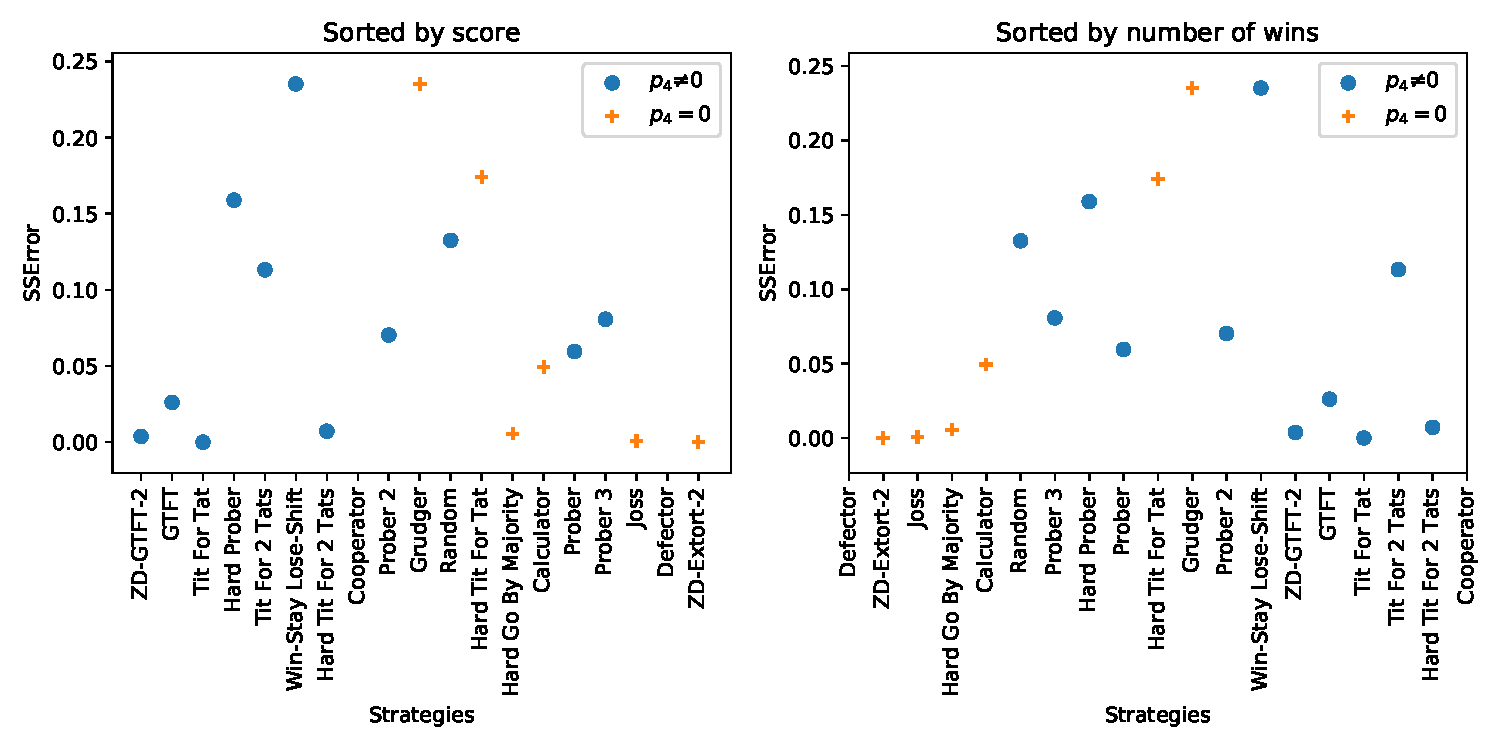
\includegraphics[width=.8\textwidth]{./assets/img/SSError_overall_in_stewart_plotkin/main.pdf}
    \caption{\(\text{SSError}\) and state probabilities for the strategies
        of~\cite{Stewart2012}, ordered both by number of wins and overall score.
        Note that \(P(DC)\) is not shown as it corresponds to the transpose of
        \(P(CD)\). Cooperator and Defector are omitted as they do not visit all
        the states.}
    \label{fig:SSError_overall_in_stewart_plotkin}
\end{figure}

Here, the work of~\cite{Stewart2012} is extended by investigating a tournament
with 204
strategies.

The results of this analysis are shown in
Figure~\ref{fig:SSError_and_probabilities_in_full}. The top ranking strategies
by number of wins seem to be extortionate (but not against all strategies) and
it can be seen that a small sub group of strategies achieve mutual defection.
All the top ranking strategies according to score achieve mutual cooperation and
do not extort each other, however they
\textbf{do} exhibit extortionate behaviour towards a number of the lower ranking
strategies.

\begin{figure}[!htbp]
    \centering
    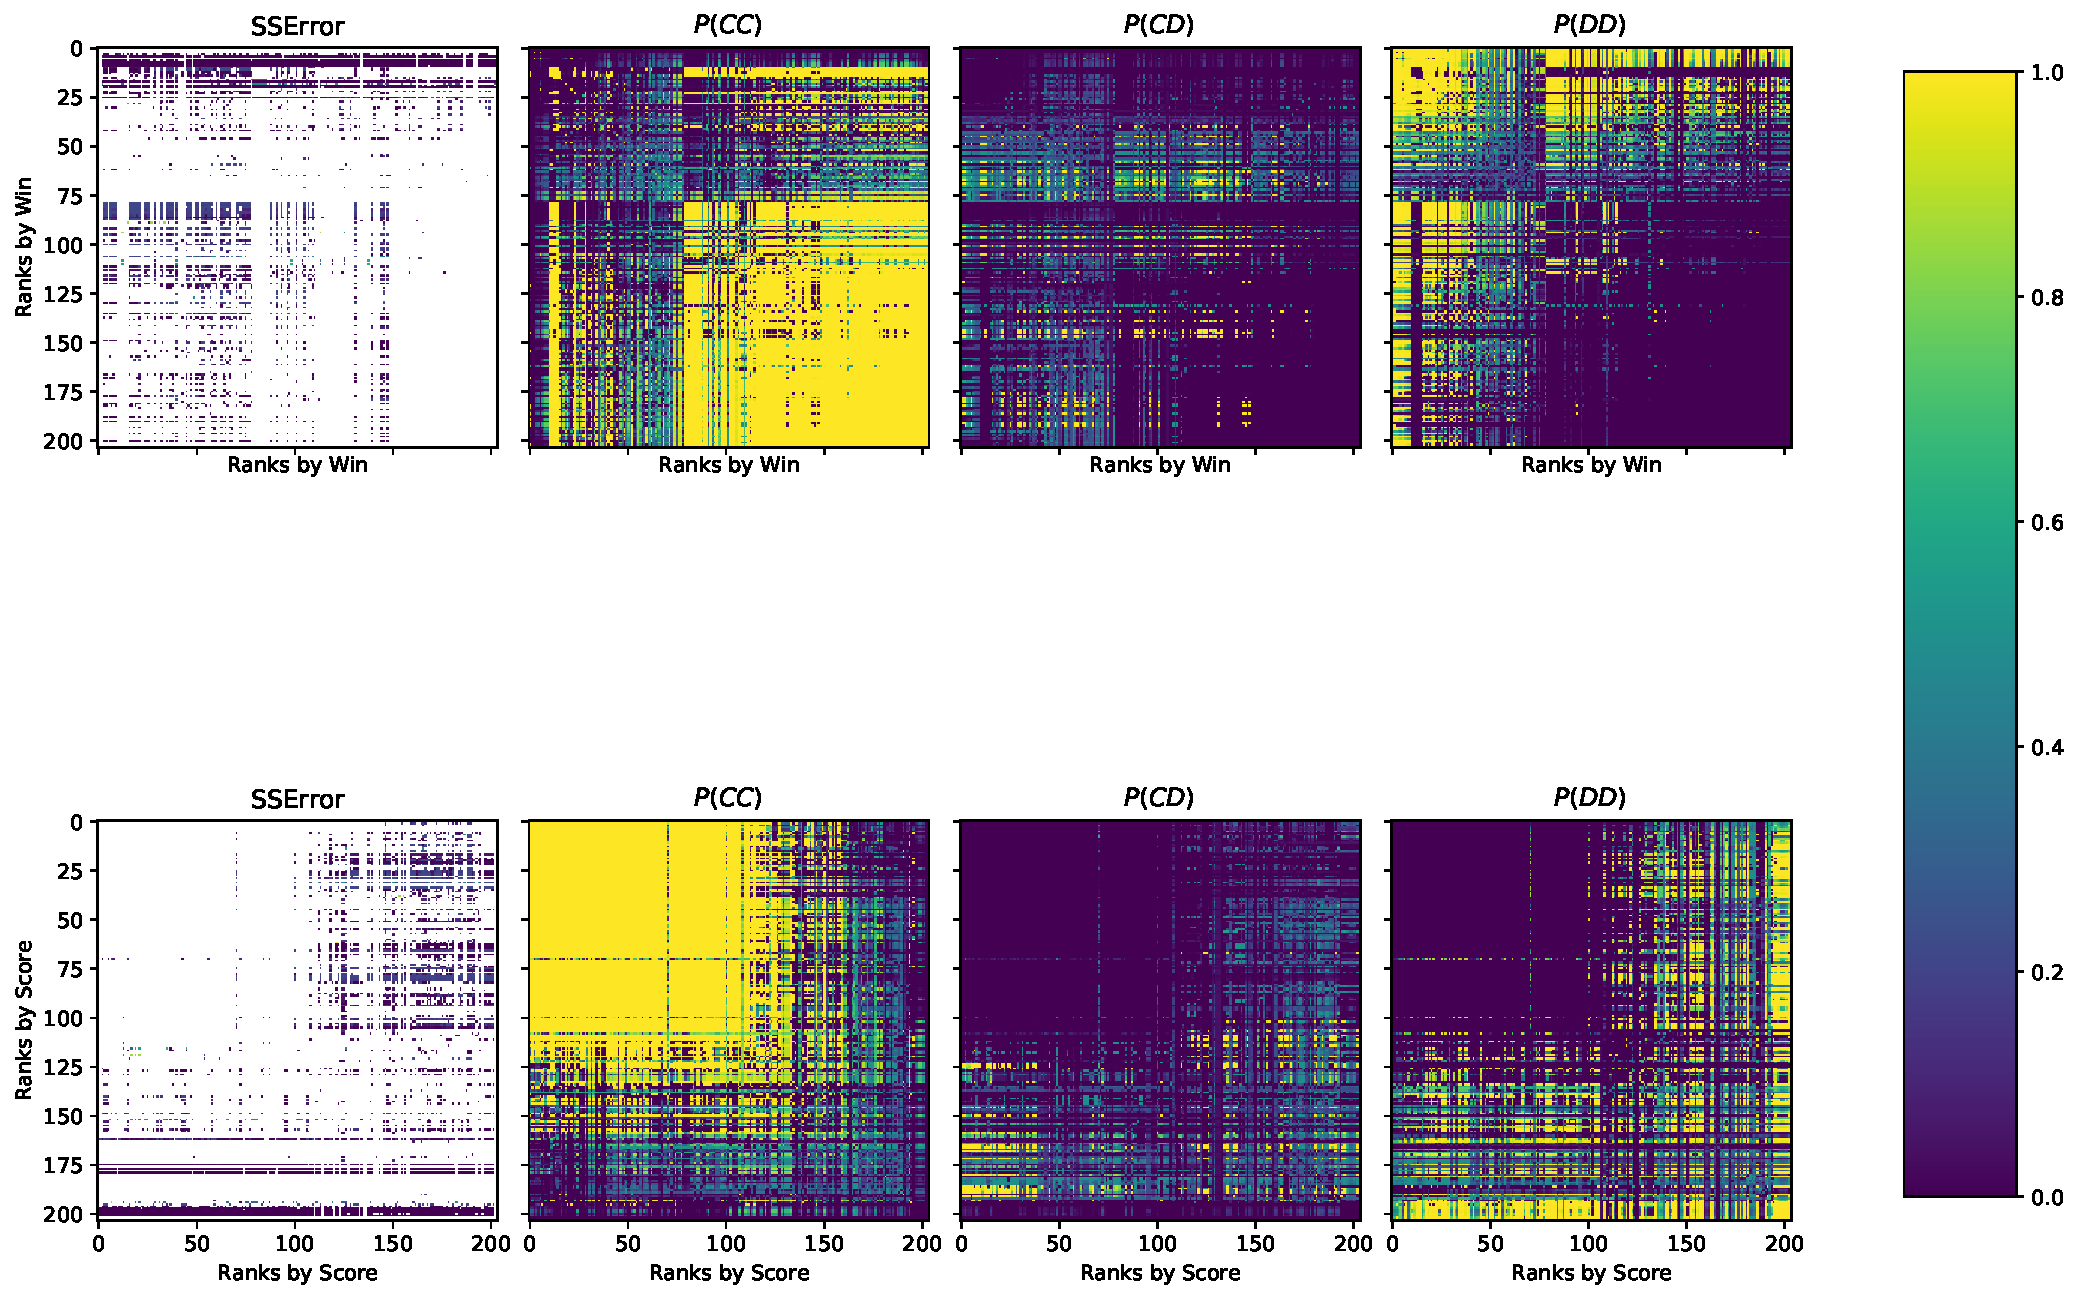
\includegraphics[width=.8\textwidth]{./assets/img/SSError_and_probabilities_in_full/main.pdf}
    \caption{\(\text{SSError}\) for the strategies for the full tournament. Only
    strategy interactions for which \(p_4=0\) and \(\chi>1\) are displayed.}
    \label{fig:SSError_and_probabilities_in_full}
\end{figure}

A detailed look at selected strategies is given in
Table~\ref{tbl:overall_summary_results}. It can be seen that \texttt{Extort-2}
wins many matches but does not achieve a high mean score or a high mutual
cooperation rate (\(P(CC)\)) but it does win most of its matches.

\begin{table}[!hbtp]
    \begin{center}
    \tiny
    \begin{tabular}{rlrrrrrrrrrrr}
\toprule
 Rank &                   Name &  Score per turn &  $P($Win$)$ &  $P(CC)$ &  Overall $\kappa$ &  Min $\kappa$ &  5\% CI $\kappa$ &  Median $\kappa$ &  Mean $\kappa$ &  Std $\kappa$ &  95\% CI $\kappa$ &  Max $\kappa$ \\
\midrule
    1 &   EvolvedLookerUp2\_2\_2 &           2.944 &       0.230 &    0.673 &             0.230 &         0.015 &           0.059 &            1.235 &          1.087 &         0.482 &            1.721 &         2.471 \\
    2 &          Evolved HMM 5 &           2.944 &       0.205 &    0.718 &             0.102 &         0.030 &           0.086 &            1.235 &          0.808 &         0.540 &            1.235 &         1.235 \\
    3 &      PSO Gambler 2\_2\_2 &           2.913 &       0.204 &    0.624 &             0.200 &         0.005 &           0.059 &            1.235 &          0.911 &         0.539 &            1.236 &         2.471 \\
    4 &       PSO Gambler Mem1 &           2.908 &       0.211 &    0.715 &             0.068 &         0.054 &           0.066 &            1.235 &          0.720 &         0.575 &            1.235 &         1.235 \\
    5 &      PSO Gambler 1\_1\_1 &           2.906 &       0.221 &    0.696 &             0.138 &         0.022 &           0.055 &            1.235 &          0.749 &         0.543 &            1.235 &         1.235 \\
    7 &          Evolved ANN 5 &           2.893 &       0.225 &    0.682 &             0.001 &         0.000 &           0.001 &            1.235 &          0.814 &         0.572 &            1.235 &         1.235 \\
   31 &              ZD-GTFT-2 &           2.721 &       0.000 &    0.806 &             0.066 &         0.020 &           0.064 &            1.235 &          0.809 &         0.538 &            1.235 &         1.235 \\
   45 &               ZD-GEN-2 &           2.689 &       0.016 &    0.801 &             0.016 &         0.003 &           0.015 &            1.235 &          0.699 &         0.599 &            1.235 &         1.235 \\
   47 &              Eatherley &           2.682 &       0.000 &    0.828 &             0.084 &         0.000 &           0.003 &            1.235 &          0.904 &         0.479 &            1.235 &         1.235 \\
   69 &            Tit For Tat &           2.638 &       0.000 &    0.723 &             0.000 &         0.000 &           0.000 &            1.235 &          0.796 &         0.564 &            1.235 &         1.235 \\
   75 &                 Grumpy &           2.630 &       0.075 &    0.793 &             0.000 &         0.000 &           0.000 &            1.235 &          0.979 &         0.492 &            1.235 &         1.235 \\
   88 &    Win-Stay Lose-Shift &           2.616 &       0.099 &    0.649 &             1.235 &         1.000 &           1.000 &            1.235 &          1.206 &         0.077 &            1.235 &         1.235 \\
  103 &  Eventual Cycle Hunter &           2.565 &       0.067 &    0.770 &             0.000 &         0.000 &           0.003 &            1.235 &          0.753 &         0.584 &            1.235 &         1.235 \\
  107 &  Tricky Level Punisher &           2.537 &       0.062 &    0.828 &             0.000 &         0.000 &           0.000 &            1.235 &          0.711 &         0.595 &            1.235 &         1.235 \\
  127 &               Adaptive &           2.272 &       0.500 &    0.363 &             0.000 &         0.000 &           0.000 &            0.059 &          0.097 &         0.222 &            0.276 &         1.529 \\
  169 &                  Bully &           1.970 &       0.381 &    0.141 &             1.529 &         0.059 &           0.209 &            1.529 &          1.411 &         0.349 &            1.529 &         1.529 \\
  179 &             Alternator &           1.945 &       0.392 &    0.157 &             1.529 &         1.000 &           1.000 &            1.529 &          1.594 &         0.344 &            2.471 &         2.471 \\
  181 &               Negation &           1.941 &       0.356 &    0.141 &             1.529 &         0.292 &           1.229 &            1.529 &          1.486 &         0.207 &            1.529 &         2.005 \\
  183 &              Cycler DC &           1.931 &       0.324 &    0.149 &             1.529 &         0.529 &           0.529 &            1.529 &          1.274 &         0.419 &            1.529 &         1.529 \\
  188 &               Hopeless &           1.908 &       0.352 &    0.261 &             2.471 &         1.009 &           1.363 &            2.471 &          2.102 &         0.429 &            2.471 &         2.471 \\
  194 &         Gradual Killer &           1.892 &       0.354 &    0.439 &             0.000 &         0.000 &           0.000 &            0.089 &          0.148 &         0.187 &            0.298 &         1.235 \\
  196 &             Aggravater &           1.879 &       0.930 &    0.087 &             0.235 &         0.059 &           0.059 &            0.059 &          0.095 &         0.065 &            0.235 &         0.235 \\
  200 &            ZD-Extort-2 &           1.821 &       0.851 &    0.179 &             0.000 &         0.000 &           0.000 &            0.000 &          0.027 &         0.160 &            0.009 &         1.059 \\
  201 &            ZD-Extort-4 &           1.820 &       0.865 &    0.106 &             0.000 &         0.000 &           0.000 &            0.000 &          0.028 &         0.157 &            0.066 &         1.237 \\
  202 &             ZD-Extort3 &           1.810 &       0.862 &    0.133 &             0.000 &         0.000 &           0.000 &            0.000 &          0.027 &         0.161 &            0.014 &         1.060 \\
  203 &               Defector &           1.808 &       0.929 &    0.000 &             0.059 &         0.059 &           0.059 &            0.059 &          0.059 &         0.000 &            0.059 &         0.059 \\
  204 &              Handshake &           1.806 &       0.870 &    0.046 &             0.000 &         0.000 &           0.000 &            0.529 &          0.511 &         0.344 &            1.236 &         1.721 \\
\bottomrule
\end{tabular}

    \end{center}
    \caption{Summary of overall results for a selected list of strategies. The
    transition rates are computed as an average over all matches.}
    \label{tbl:overall_summary_results}
\end{table}

\section{Conclusion}\label{sec:conclusion}

This work defines an approach to measure whether or not a player is playing a
strategy that corresponds to an extortionate strategy as defined
in~\cite{Press2012}: a mathematical model for suspicion. Indeed, all
extortionate strategies have been classified as lying on a triangular plane.
This rigorous classification fails to be robust to small measurement error, thus
a statistical approach is proposed.
This is done through a linear algebraic approach for approximating the solution
of a linear system. Using this, a large number of pairwise interactions is
simulated and in fact very few strategies are found to act extortionately.

The work of~\cite{Press2012}, whilst showing that a clever approach to taking
advantage of another memory one strategy exists: this is incomplete. Whilst the
elegance of this result is very attractive, just as the simplicity of the
victory of Tit For Tat in Axelrod's original tournaments was, it is incomplete.
Extortionate strategies achieve a high number of wins but they do not
achieve a high score which corresponds to the fitness landscape in an
evolutionary sense. From the large number of interactions a payoff matrix \(S\)
can be measured where \(S_{ij}\) denotes the score (using standard values of
\((R, S, T, P) = (3, 0, 5, 1)\)) of the \(i\)th strategy
against the \(j\)th strategy. Using this, the replicator equation
describes the evolution of the system based on a population density fitness
function:

\begin{equation}\label{eqn:replicator_dynamics}
    \frac{dx}{dt} = x(S-x^TS x)
\end{equation}

Equation (\ref{eqn:replicator_dynamics}) is solved numerically through an
integration technique described in~\cite{Petzold1983} and
Figure~\ref{fig:replicator_dynamics} shows the evolution of the distribution of
the system: the various strategies are ranked by scores. It is clear to see that
only the high ranking strategies survive the evolutionary process (in fact,
only 39
have a final distribution value greater than \(10 ^ {-2}\)). This confirms the
findings of~\cite{Moran1707} in which sophisticated strategies resist
evolutionary invasion of shorter memory strategies. Recalling
Figure~\ref{fig:SSError_and_probabilities_in_full} this demonstrates that:

\begin{itemize}
    \item Cooperation emerges through the evolutionary process: the high scoring
        strategies do not exhibit extortionate behaviour towards each other.
    \item Extortionate strategies do not survive the evolutionary process.
\end{itemize}

\begin{figure}[!htbp]
    \centering
    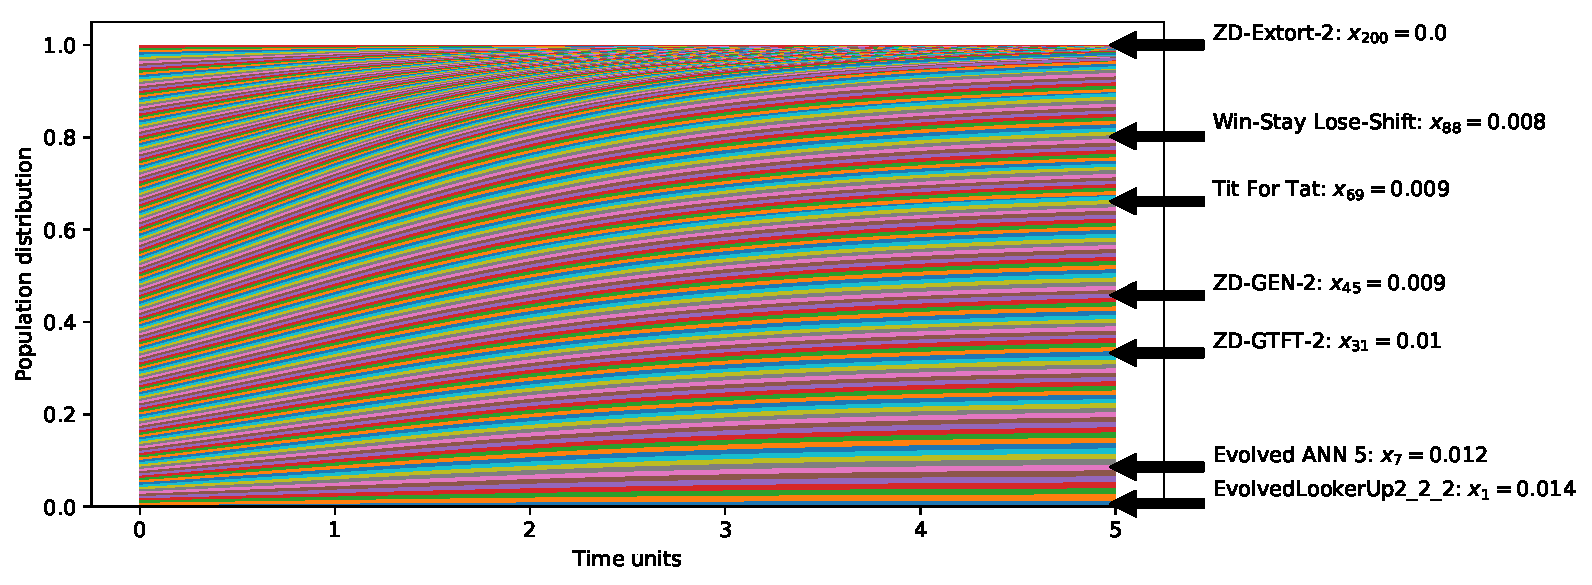
\includegraphics[width=.8\textwidth]{./assets/img/replicator_dynamics/main.pdf}
    \caption{Numerical simulation of the replicator equation
    (\ref{eqn:replicator_dynamics}): strategies are ordered by score. Some
    selected strategies are highlighted with their long run population
    distribution.}
    \label{fig:replicator_dynamics}
\end{figure}

This work can be used to classify plays of the IPD\@: data can be collected from
actual interactions (in lab or in the field). Furthermore, this allows for a
classification method similar to the notion of fingerprinting presented
in~\cite{Ashlock2008}. Trained strategies can potentially be classified as
extortionate or not or it could be possible to even constrain the reinforcement
learning approaches that are becoming prevalent in the literature.
Alternatively, this mathematical approach for recognising extortion could be
used in sophisticated strategies to defend against invasion. Arguably, some of
the strategies considered here exhibit this behaviour, indeed as described
in~\cite{Harper2017}, the top ranking strategies in the full tournament are
obtained using evolutionary reinforcement learning techniques, thus, suspicion
of extortionate behaviour could in fact be an evolutionary trait.

\section*{Acknowledgements}

The following open source software libraries were used in this research:

\begin{itemize}
    \item The Axelrod ~\cite{Knight2016, Knight2018} library (IPD strategies and
        tournaments).
    \item The sympy library~\cite{Meurer2017} (verification of all symbolic
        calculations).
    \item The matplotlib~\cite{Droettboom2018} library (visualisation).
    \item The pandas~\cite{Structures2010}, dask~\cite{Dask2016} and
        NumPy~\cite{Oliphant2015} libraries (data manipulation).
    \item The SciPy~\cite{Jones2001} library (numerical integration of the
        replicator equation).
\end{itemize}

This work was performed using the computational facilities of the Advanced
Research Computing @ Cardiff (ARCCA) Division, Cardiff University.

\printbibliography

\newpage
\section*{Supplementary materials}

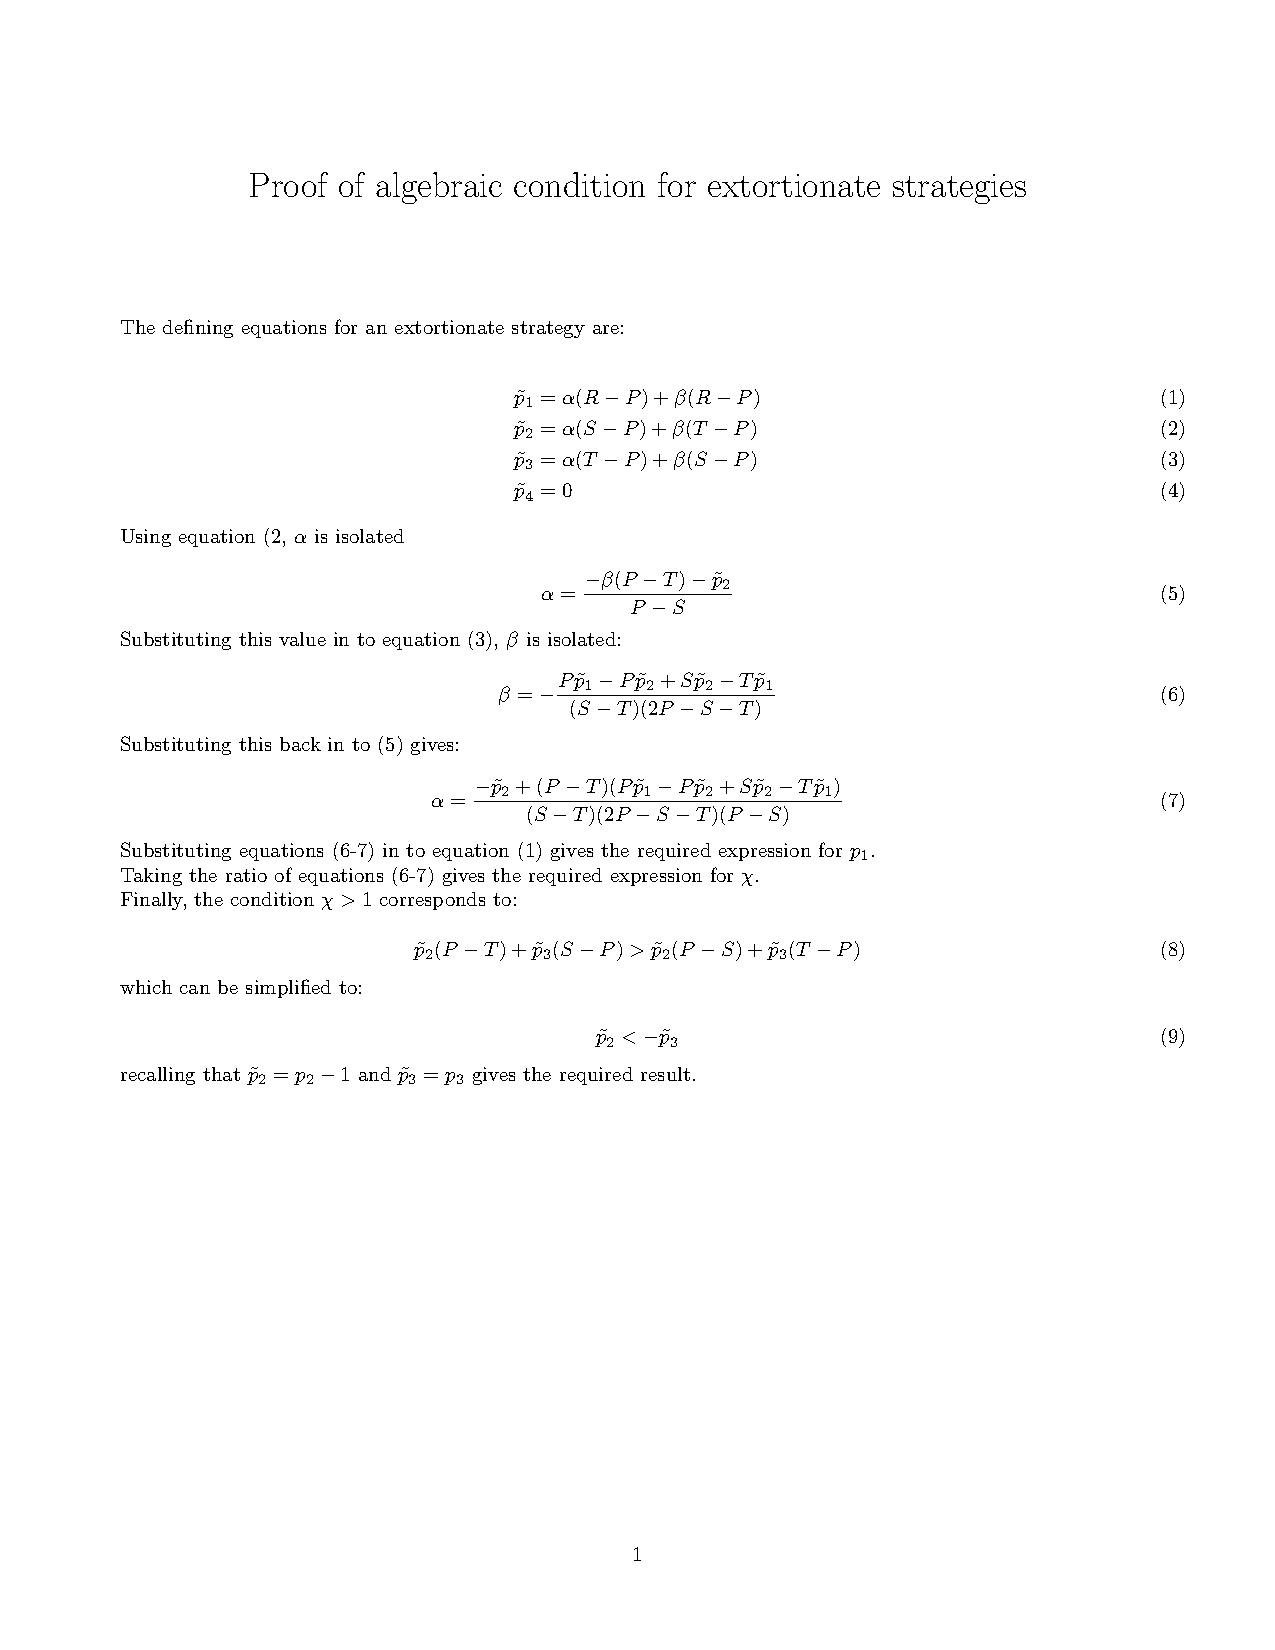
\includepdf{assets/pdf/proof_of_form_of_extortionate_strategies/main.pdf}

\newpage

Using the pair wise interactions the transition rates \(p,
q\) can be measured and the steady state probabilities inferred and compared to
the actual probabilities of each state.
This is done numerically by computing the singular eigenvector of the
matrix \(A\) \cite{Stewart2009}:

\[
    A =
    \begin{bmatrix}
        p_1 q_1 & p_1 (1 - q_1) & (1 - p_1) q_1 & (1 -p_1) (1 - q_1) \\
        p_2 q_2 & p_2 (1 - q_2) & (1 - p_2) q_2 & (1 -p_2) (1 - q_2) \\
        p_3 q_3 & p_3 (1 - q_3) & (1 - p_3) q_3 & (1 -p_3) (1 - q_3) \\
        p_4 q_4 & p_4 (1 - q_4) & (1 - p_4) q_4 & (1 -p_4) (1 - q_4) \\
    \end{bmatrix}
\]

Figure~\ref{fig:computed_probabilities_vs_theoretic_probabilities} shows a
regression line fitted to every pairwise interaction with a reported
\(\text{SSError}\) value (pairwise interactions with missing states were
omitted). This serves to validate the approach: a part from some edge cases the
relationship is consistent.

\begin{figure}[!htbp]
    \centering
    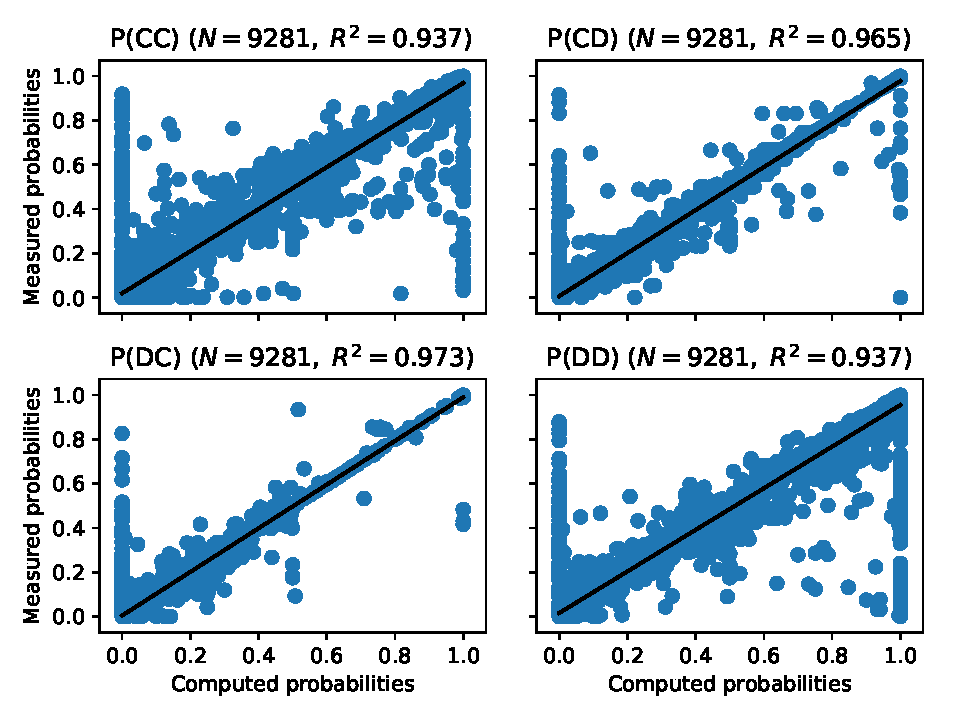
\includegraphics[width=.8\textwidth]{./assets/img/computed_probabilities_vs_theoretic_probabilities/main.pdf}
    \caption{The
        relationship between the steady state probabilities inferred from the
        measured transitions and the actual steady state probabilities. A linear
        regression line is included validating the approach.}
    \label{fig:computed_probabilities_vs_theoretic_probabilities}
\end{figure}


\end{document}
